%
% OK, here is the rough plan I though about
%
%
% 10/15 minutes introduction explaining what is a UAV/UAS, autonomous fligh, 
% what we are going to do during the flight
%
% 15/30 minutes flight
%
% rest should be scalable between 15 and 45 minutes depending on how the flight goes
%
% -paparazzi project
%
% -hardware
%   -airframe
%   -avionics 
%     -CPU
%     -sensors
%     -communications
%     -payloads
%
%
% -software
%   -flight plan language
%   -networked architecture
%   -payload (pan tilt camera, balldrop, chemo sensor...)
%   -
%
%
% -applications/results
%   -reglementation
%   -teaching/research
%   -rt benchmark
%   -mav competitions
%   -iceland
%   -forest fire
%
% -conclusion
%
%
\documentclass{beamer}
\usepackage{graphicx}
\usepackage{calc}

\graphicspath{{../images/},{tmp/}}
%\usetheme{shadow}
\usetheme{Singapore}
\useoutertheme{infolines}
\usecolortheme{seahorse}
\useinnertheme[shadow]{rounded}
\setbeamercolor{block title}{bg=black!10!white}

\usepackage{xmpmulti}
\DeclareGraphicsRule{*}{mps}{*}{}

\usepackage{multimedia}
\title{\movie[externalviewer]{Build your own UAV}{../videos/intro.avi}}
\author{M. Mueller, A. Drouin}
\date{December 2007}
\institute{
%\inst{1}%
Bosh/ENAC
}
%\titlegraphic{\includegraphics[height=2cm]{Aircrafts/Multiple/avions_enac}}
\pgfdeclareimage[height=1cm]{penguin}{../images/logos/penguin}
\pgfdeclareimage[height=1cm]{enac}{../images/logos/logo_enac}

\setbeamertemplate{frametitle}
{
\begin{beamercolorbox}{frametitle}
\begin{centering}
\pgfuseimage{enac} \hfill \raisebox{0.3cm}{\textbf{\insertframetitle}}\hfill \pgfuseimage{penguin}
\par
\end{centering}
\end{beamercolorbox}
}


% \setbeamertemplate{itemize item}{$\Rightarrow$}

\begin{document}
\maketitle


\frame{\tableofcontents}


%
% Overview
%
\section{Introduction}
\begin{frame}
  \frametitle{UAV}

  \begin{center}
    \includegraphics[height=6cm]{misc_uavs/global_hawk}<1>
    \includegraphics[height=6cm]{misc_uavs/predator}<2>
    \includegraphics[height=6cm]{misc_uavs/raven}<3>
    \includegraphics[height=6cm]{misc_uavs/missile}<4>
    \includegraphics[height=6cm]{misc_uavs/weather_balloon}<5>
  \end{center}
\end{frame}




\begin{frame}
  \frametitle{UAS}

  \begin{center}
    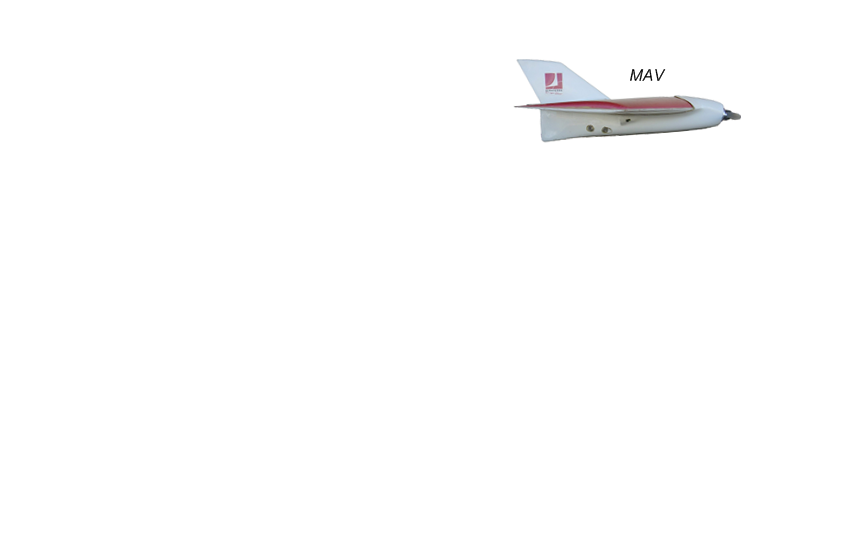
\includegraphics[height=6cm]{system/system_overview_0}<1>
    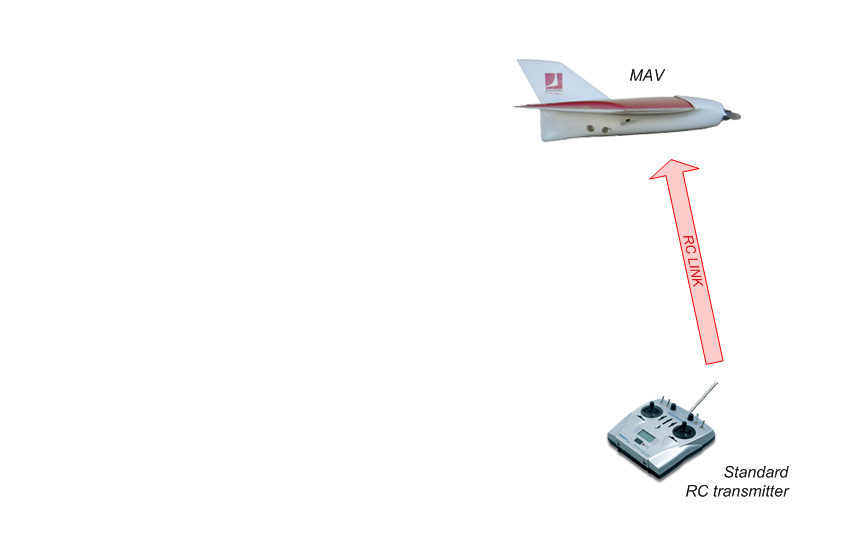
\includegraphics[height=6cm]{system/system_overview_1}<2>
    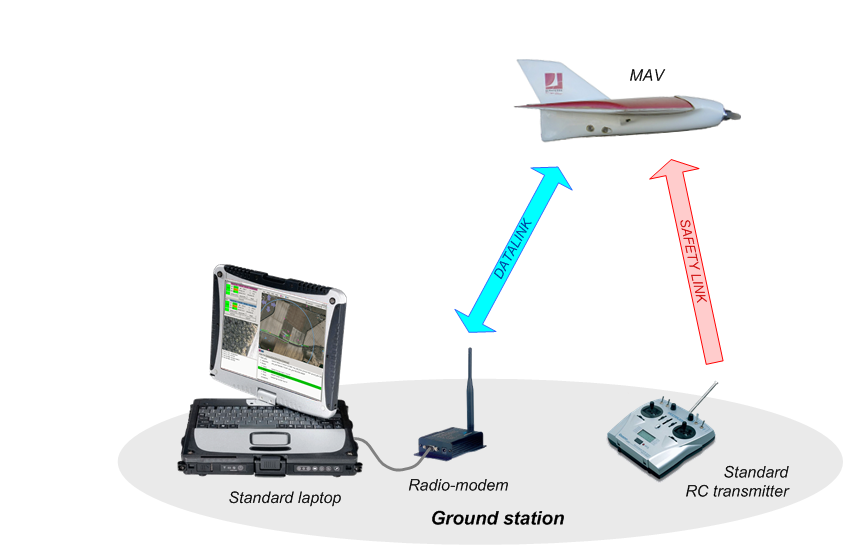
\includegraphics[height=6cm]{system/system_overview_2}<3>
    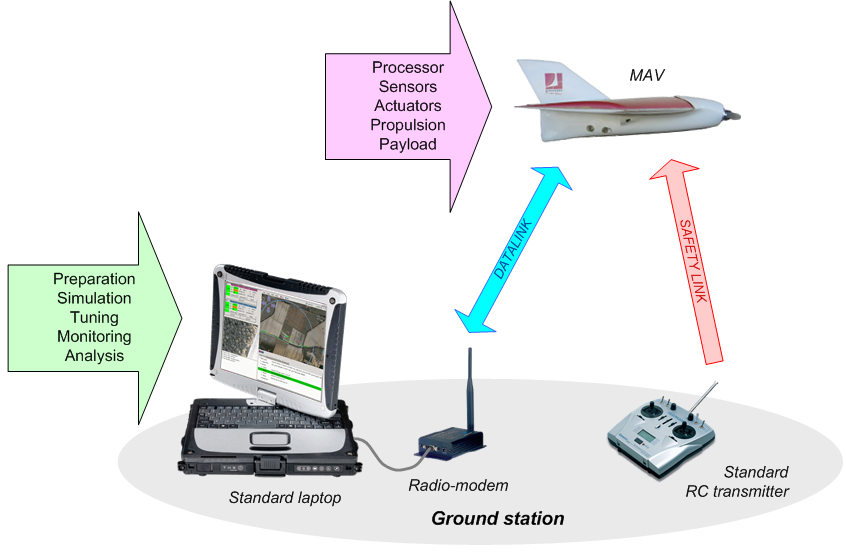
\includegraphics[height=6cm]{system/system_overview_3}<4>
  \end{center}
\end{frame}

%
% Features
%
\subsection{Features}

% control
% - augmented stability
% - waypoint navitation
% - complex trajectories
% - dynamic trajectories ( search patterns )


%
% Networked architecture
\begin{frame}
\frametitle{Architecture}
\begin{center}
Multi-aircraft network enabled ground segment
\end{center}
\begin{center}
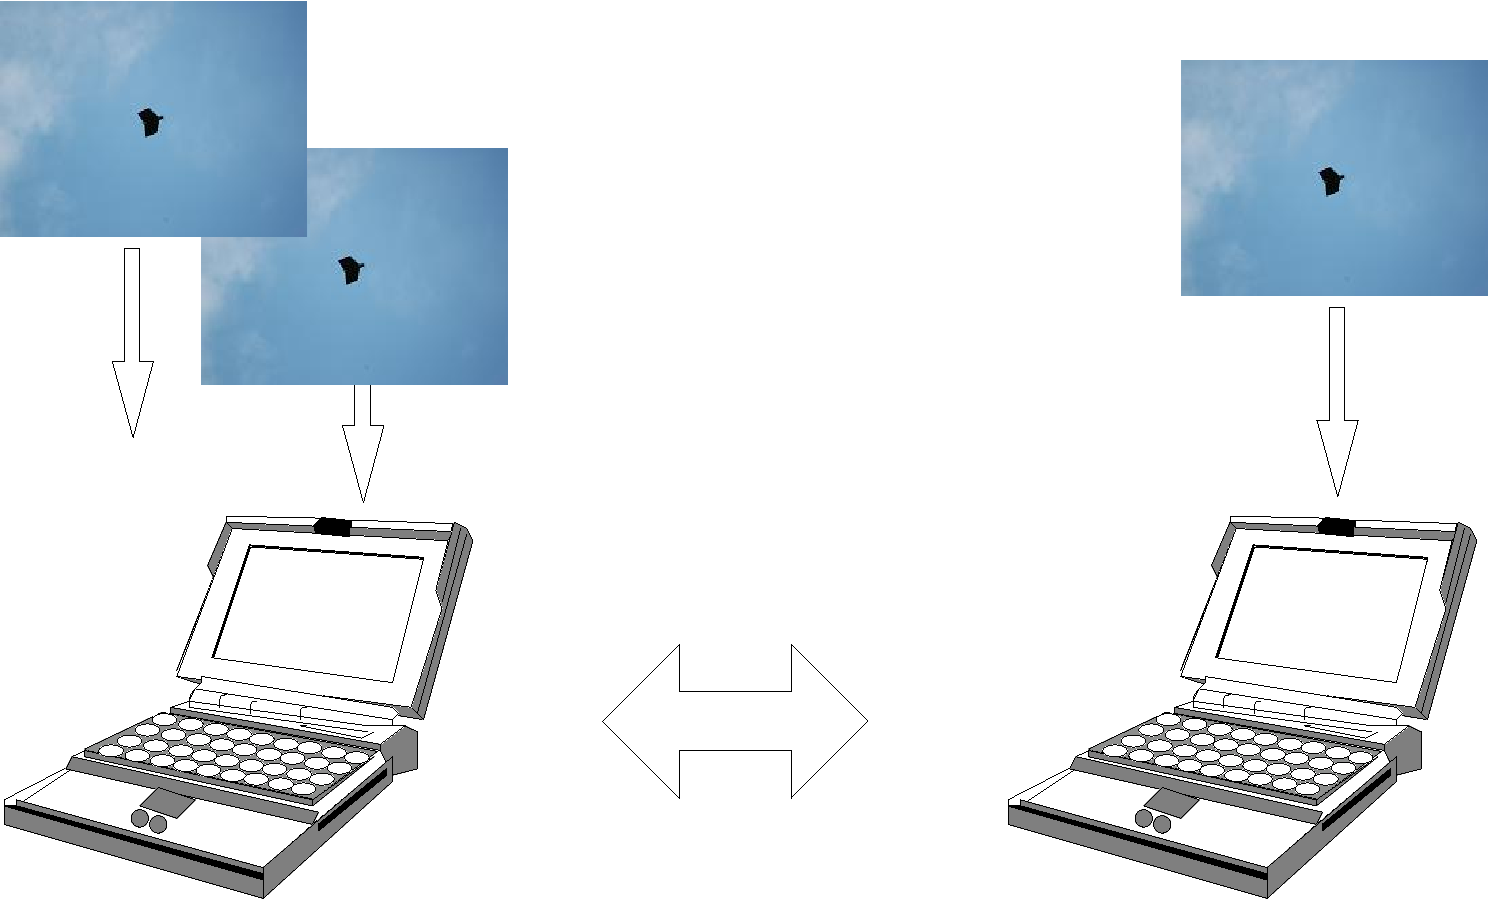
\includegraphics[height=4cm]{system/network}
\end{center}
\end{frame}


% configuration
% simulation
% flight
% analysis
% replay


%
% Ground station
\begin{frame}
  \frametitle{Multi-UAV Human Machine Interface}

  \begin{center}
    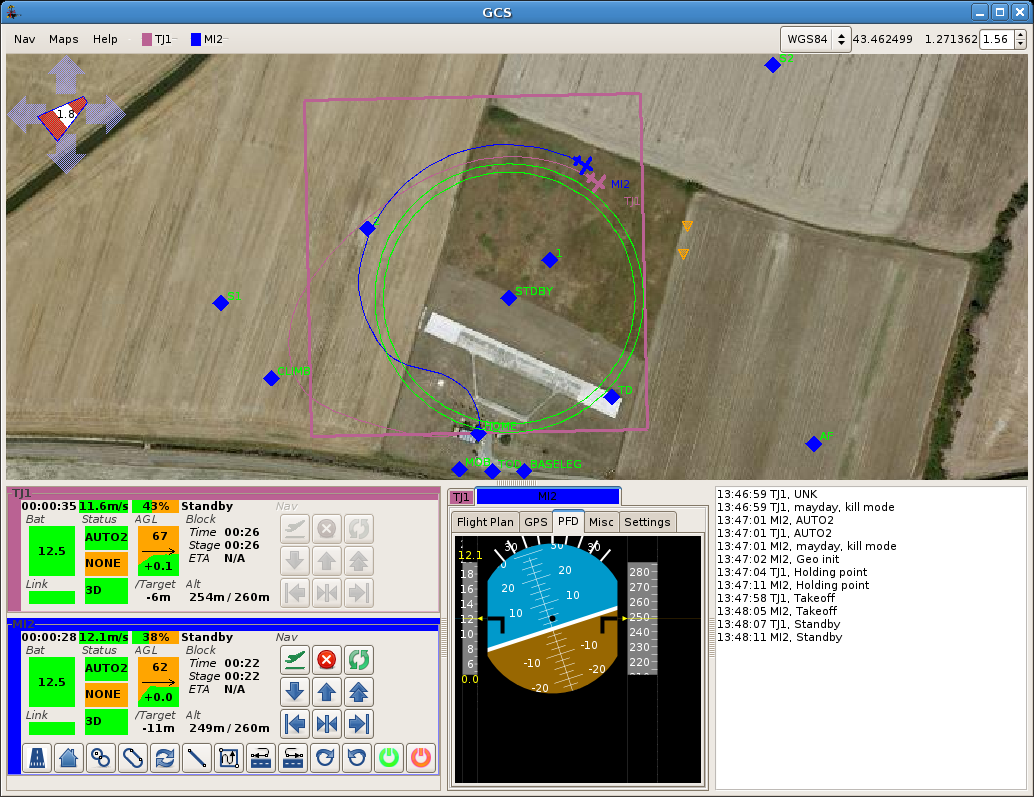
\includegraphics[height=7cm]{gcs/overall}
  \end{center}
\end{frame}


%
% Control board
\begin{frame}
  \frametitle{Controller board}
  \begin{center}
    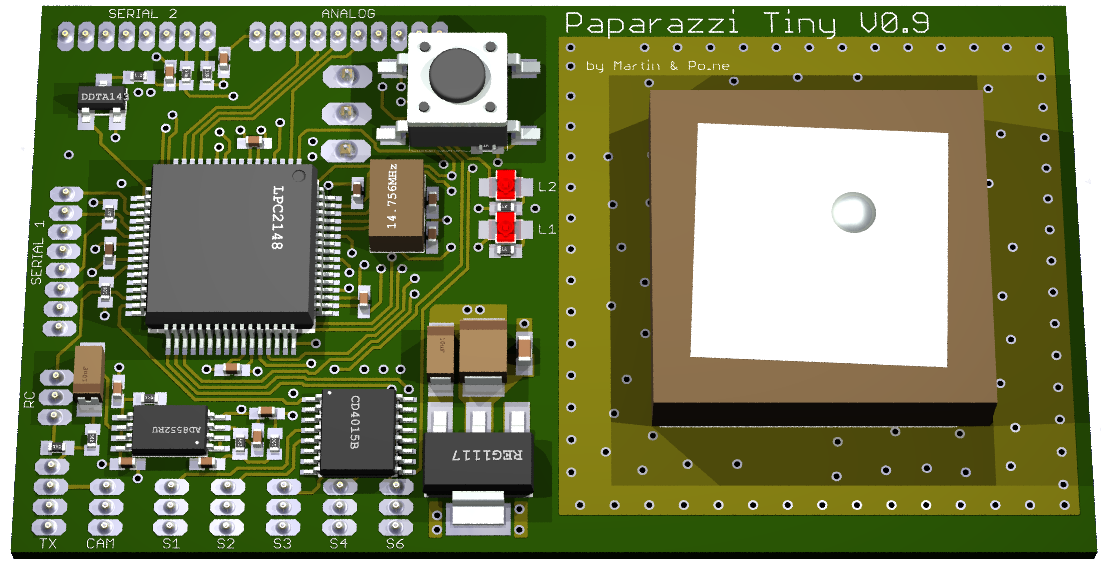
\includegraphics[width=7cm]{control_board/tiny_cad_top.png}
   
    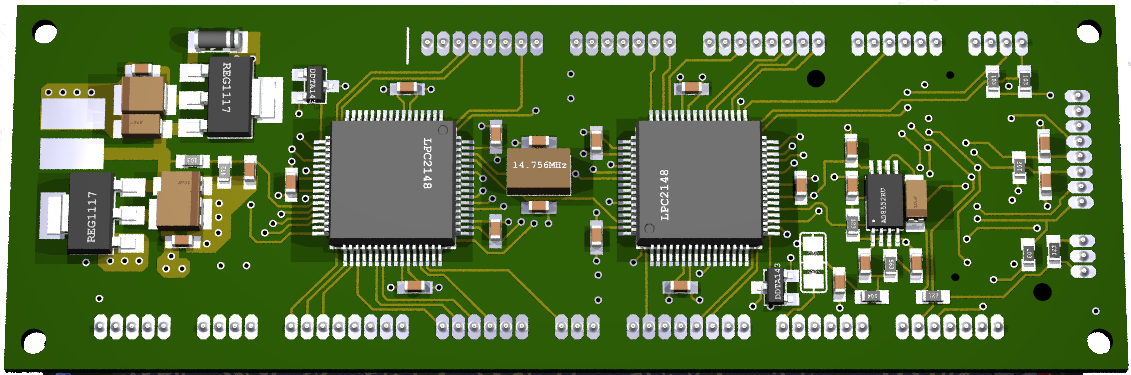
\includegraphics[width=8cm]{control_board/classix_cad_top.png}    
  \end{center}
\end{frame}


%
% Sensors



%
% Video
\begin{frame}
\frametitle{Video}

\begin{columns}
\begin{column}{5cm}
\begin{itemize}
\item Real-time video downlink
\item Footprint on map
\item Network streaming
\item Stitching
\item Smoke detection
\end{itemize}
\end{column}
\begin{column}{5cm}
\begin{center}
\movie[externalviewer=gxine]{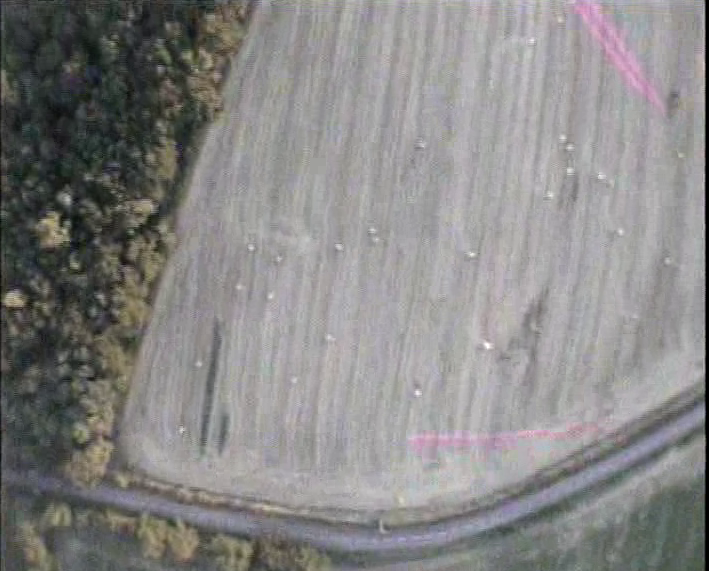
\includegraphics[height=3cm]{aerial/montfaucon}}{../video/montfaucon.avi}
\end{center}
\end{column}
\end{columns}
\begin{center}
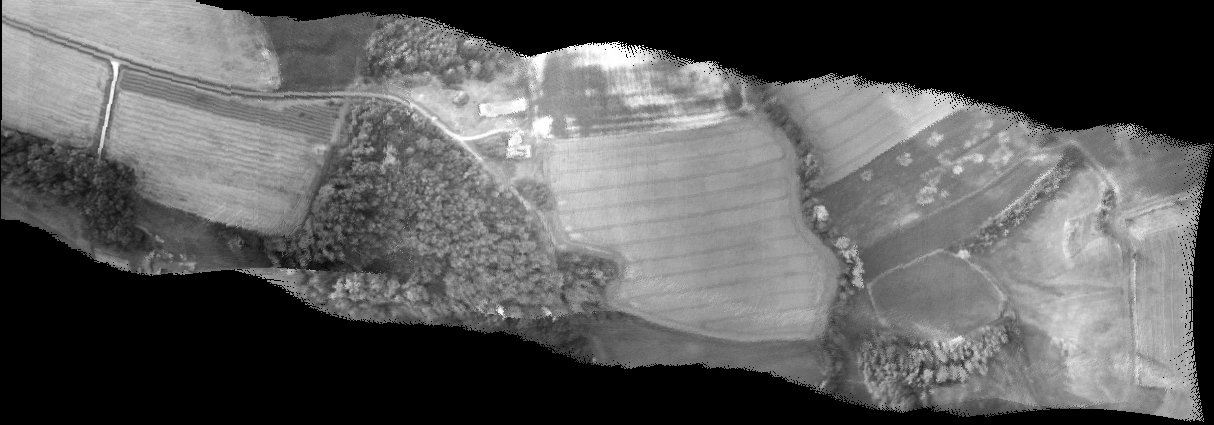
\includegraphics[width=9cm]{aerial/collage_adrien}<1>
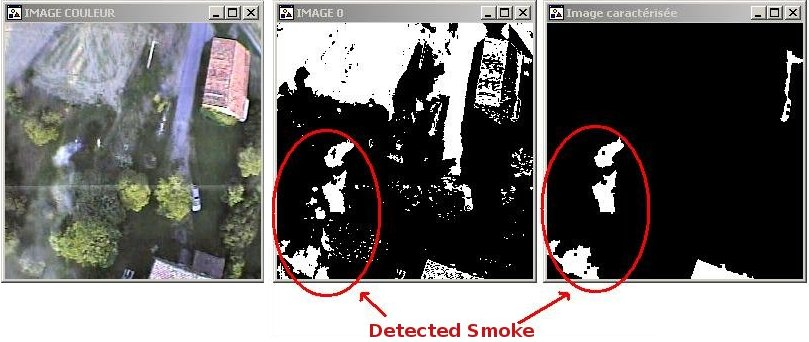
\includegraphics[width=9cm]{aerial/video8}<2>
\end{center}
\end{frame}


%
% History
%
\subsection{History}


%
%
% Flight demo
%
%
\section{Flight Presentation}

%
% Project
%
\section{Paparazzi Project}





%
% Hardware
%
\section{Hardware}




%
% Software
%
\section{Software}




%
% Applications
%
\section{Applications}
\begin{frame}
  \frametitle{MAV Competitions}
    \begin{itemize}
      \item JMD03, Toulouse, France: 1st place with the Twinstar
      \item EMAV04, Braunschweig, Germany: 1st place with the Microjet
      \item JMD04, Toulouse, France: 1st place with the Microjet
      \item MAV05, Garmisch, Germany: 4 Paparazzi teams at the first 4 places
      \item EMAV06, Braunschweig, Germany : all the teams were equiped with Paparazzi
      \item MAV06, Sandestin, Florida: 2nd and 3rd places
      \item MAV07, Toulouse, France: 1st place (tie), 3rd, 4th and 5th places
    \end{itemize}
\end{frame}

\begin{frame}
  \frametitle{Teaching/Reasearch}
% in the UAV field ( structure/propulsion/control etc... )
% in other aeronautics fields as an affordable aircraft substitute
% data collection (environment/video/meteo )
% as an application in even farther fields (formal methods/ real time benchmark )
\end{frame}

\begin{frame}
  \frametitle{Forest fire detection}


\end{frame}


\begin{frame}
  \frametitle{Meteorological surveying}
    \begin{center}
      \includegraphics[height=6cm]{applications/kerlingafjoll}<1>
      \includegraphics[height=6cm]{applications/high_alt}<2>
  \end{center}	

\end{frame}


%
% Conclusions
%
\section{Conclusions}

\begin{frame}
  \frametitle{Conclusions}
    \begin{itemize}
      \item<1-> COTS + Free Software enable affordable mini/micro UAVs
      \item<2-> Wide fields of applications
      \item<3-> Reglementation lagging
    \end{itemize}
\end{frame}

\begin{frame}
  \frametitle{Acknowledments}
  \begin{columns}
    \begin{column}{5cm}
	\begin{itemize}
	  \item<1-> Pascal Brisset
	  \item<2-> Murat Bronz
	  \item<3-> Michel Gorraz
	  \item<4-> Anton Kochevar
	  \item<5-> Christian Lindenberg
	  \item<6-> Arnorld XXX
	  \item<7-> Jeremy Tyler
	  \item<7-> and all others...
        \end{itemize}
    \end{column}

    \begin{column}{5cm}
      \begin{center}
        \includegraphics[height=6cm]{team/frozen_pascal}<1>
        \includegraphics[height=6cm]{team/murat}<2>
        \includegraphics[height=6cm]{team/michel}<3>
        \includegraphics[height=6cm]{team/anton}<4>
        \includegraphics[height=6cm]{team/christian}<5>
        \includegraphics[height=6cm]{team/arnold}<6>
        \includegraphics[height=6cm]{team/jeremy}<7>
      \end{center}
    \end{column}
  \end{columns}
\end{frame}


\begin{frame}
  \frametitle{Further Informations}

  %\movie[externalviewer]{\includegraphics[width=4cm]{penguin_logo}}{../video/outro.avi}
  %~\hfill~
  
\includegraphics[width=4cm]{penguin}

    \begin{itemize}
      \item \url{http://paparazzi.nongnu.org}
      \item \url{http://paparazzi.enac.fr}
      \item \url{irc://irc.freenode.net/#paparazzi}
    \end{itemize}

\end{frame}





\frame{} % to enforce entries in the table of contents

\end{document}
